\chapter{貪欲アルゴリズム - Greedy algorithms}

\index{貪欲アルゴリズム -greedy algorithm}

A \key{貪欲アルゴリズム -greedy algorithm}は、
常にその時点で最善と思われる選択をすることで、問題の解を構築する方法の総称です。
貪欲なアルゴリズムは選択を取り消すことはなく、最終的な解を次々に直接構築していきます。
このため、貪欲アルゴリズムは非常に効率的に動作します。

貪欲アルゴリズムの設計で難しいのは、常に問題の最適解を生成すると保証できるアルゴリズムを見つけ出すことです。
貪欲アルゴリズムにおける局所的に最適な選択は大域的にも最適でなければならないからです。
貪欲なアルゴリズムを証明するのはしばしば困難でもあります。

\section{コイン問題 - Coin problem}

コインの組が与えられ金額$n$を形成する問題を考えましょう。
コインの値は$\texttt{coins}=\{c_1,c_2,\ldots,c_k\}$であり,
各コインは何度でも使用することができとします。
必要なコインの最小枚数は何枚か?

例えば、コインがユーロコイン(単位はセント)で、

\[\{1,2,5,10,20,50,100,200\}\]
のコインがあるとします。$n=520$だとします。最適解は$200+200+100+20$と少なくとも4枚のコインが必要になります。

\subsubsection{貪欲なアルゴリズム - Greedy algorithm}

この問題に対する貪欲アルゴリズムでは必要な金額が構成されるまで、
常に可能な限り大きなコインを選択していきます。
まず200セント硬貨を2枚選び、次に100セント硬貨を1枚、
最後に20セント硬貨を1枚選ぶので、このアルゴリズムはうまく動作するように見えます。
しかし,このアルゴリズムは常に正しく動作するのでしょうか?

コインがユーロコインであれば、
貪欲アルゴリズムが\emph{常に}機能すること、すなわち、コインの枚数が最も少ない解を常に生成することが判明しています。
このアルゴリズムの正しさは、以下のように示されます。

各コイン1, 5, 10, 50, 100が最適解に現れるのはせいぜい1回で、
もし解にそのようなコインが2枚含まれていれば次のように1枚ずつ減らし、よりよい解を得ることができるからです。
例えば、解答にコイン$5+5$が含まれている場合、$10$に置き換えることができます。

同様に、2と20が最適解に現れるのは最大2回で、
コイン$2+2+2$をコイン$5+1$、
コイン$20+20+20$をコイン$50+10$と置き換えられます。
また、$2+2+1$ や、 $20+20+10$の場合、$5$や$50$で置き換えられます。

これらのことから、各コイン$x$について、$x$より小さいコインだけを用いて最適に和$x$またはそれ以上の和を構成することは不可能であることを示すことができます。
例えば、$x = 100$の場合、小さいコインを使った最大の最適和は$50+20+20+5+2+2 = 99$である。したがって、常に最大のコインを選択する貪欲なアルゴリズムが最適解を生成します。
このようにアルゴリズム自体が単純であっても、
貪欲なアルゴリズムが有効であることを主張するのは難しいことがわかる。

\subsubsection{貪欲法でのコイン問題の一般化 - General case}

一般的な場合、コインセットには任意のコインを入れることができ、貪欲アルゴリズムは、必ずしも最適解が得られるとは限りません。

貪欲なアルゴリズムが働かないことは、アルゴリズムが間違った答えを出す反例を示すことで証明できます。
単純な例ではコインを$\{1,3,4\}$とし、目標を6としましょう。
最適解は$3 + 3$であるのに
貪欲アルゴリズムは解$4 + 1 + 1$を生成しまいます。

一般的なコイン問題がどのような貪欲アルゴリズムで解けるかは不明です。\footnote{However, it is possible
to \emph{check} in polynomial 
if the greedy algorithm presented in this chapter works for
a given set of coins \cite{pea05}.}。
しかし、第7章で見るように、常に正しい答えを与える動的計画法を使うと一般的な問題も効率的に解くことができます。

\section{スケジューリング問題 - Scheduling}

多くのスケジューリング問題も、貪欲アルゴリズムで解くことができ、古典的な問題としては以下のようなものです。
$n$個のイベントとその開始時刻と終了時刻が与えられたとき、
できるだけ多くのイベントを含むスケジュールを求めよ。
ただし、イベントを部分的に選択することはできない。

例えば、次のようなイベントを考えられます。
\begin{center}
\begin{tabular}{lll}
イベント名 & 開始時刻 & 終了時刻 \\
\hline
$A$ & 1 & 3 \\
$B$ & 2 & 5 \\
$C$ & 3 & 9 \\
$D$ & 6 & 8 \\
\end{tabular}
\end{center}

この場合は最大2つで$B$と$D$を次のように選択すればよいです。
\begin{center}
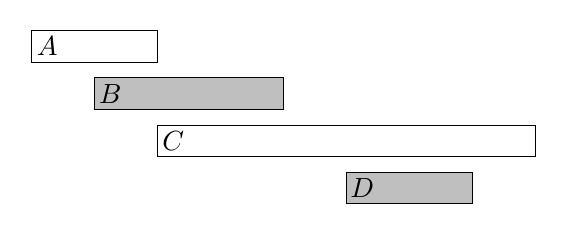
\begin{tikzpicture}[scale=.4]
  \begin{scope}
    \draw (2, 0) rectangle (6, -1);
    \draw[fill=lightgray] (4, -1.5) rectangle (10, -2.5);
    \draw (6, -3) rectangle (18, -4);
    \draw[fill=lightgray] (12, -4.5) rectangle (16, -5.5);
    \node at (2.5,-0.5) {$A$};
    \node at (4.5,-2) {$B$};
    \node at (6.5,-3.5) {$C$};
    \node at (12.5,-5) {$D$};
  \end{scope}
\end{tikzpicture}
\end{center}
どのようなアルゴリズムが考えられ、どのようなものが最適なのでしょうか?

\subsubsection*{方法1: Algorithm 1}

最初に思い浮かぶのは最も短いイベントを選ぶことです。
\begin{center}
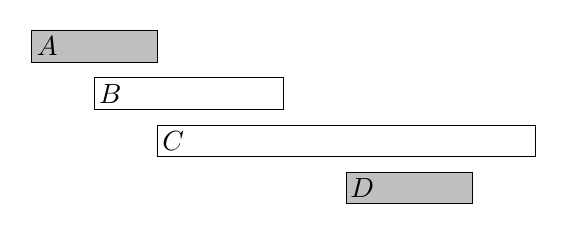
\begin{tikzpicture}[scale=.4]
  \begin{scope}
    \draw[fill=lightgray] (2, 0) rectangle (6, -1);
    \draw (4, -1.5) rectangle (10, -2.5);
    \draw (6, -3) rectangle (18, -4);
    \draw[fill=lightgray] (12, -4.5) rectangle (16, -5.5);
    \node at (2.5,-0.5) {$A$};
    \node at (4.5,-2) {$B$};
    \node at (6.5,-3.5) {$C$};
    \node at (12.5,-5) {$D$};
  \end{scope}
\end{tikzpicture}
\end{center}

ところがこれは失敗するケースがあります。反例を示します。
\begin{center}
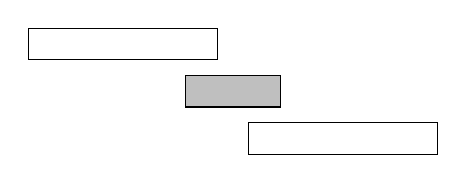
\begin{tikzpicture}[scale=.4]
  \begin{scope}
    \draw (1, 0) rectangle (7, -1);
    \draw[fill=lightgray] (6, -1.5) rectangle (9, -2.5);
    \draw (8, -3) rectangle (14, -4);
  \end{scope}
\end{tikzpicture}
\end{center}
短いイベントを選ぶと1つしか選択できませんが、実際には長い2つを取ることが出来ることは明らかです。

\subsubsection*{方法2: Algorithm 2}

では、なるべく早い時間に始まるイベントを選び続けるのはどうでしょう?
\begin{center}
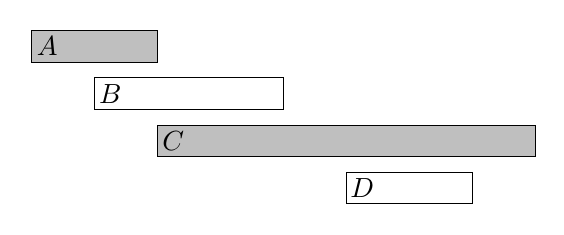
\begin{tikzpicture}[scale=.4]
  \begin{scope}
    \draw[fill=lightgray] (2, 0) rectangle (6, -1);
    \draw (4, -1.5) rectangle (10, -2.5);
    \draw[fill=lightgray] (6, -3) rectangle (18, -4);
    \draw (12, -4.5) rectangle (16, -5.5);
    \node at (2.5,-0.5) {$A$};
    \node at (4.5,-2) {$B$};
    \node at (6.5,-3.5) {$C$};
    \node at (12.5,-5) {$D$};
  \end{scope}
\end{tikzpicture}
\end{center}

これも反例が簡単に見つかってしまいます。
\begin{center}
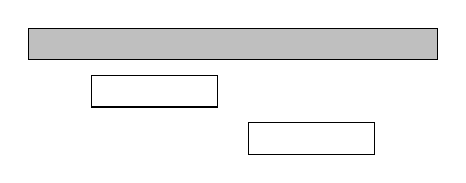
\begin{tikzpicture}[scale=.4]
  \begin{scope}
    \draw[fill=lightgray] (1, 0) rectangle (14, -1);
    \draw (3, -1.5) rectangle (7, -2.5);
    \draw (8, -3) rectangle (12, -4);
  \end{scope}
\end{tikzpicture}
\end{center}

最初のイベントを選択すると、他のイベントを選択することはできません。しかし、他の2つのイベントを選択することは可能です。

\subsubsection*{Algorithm 3}

そこで3つ目のアイデアとしては、最も早く終わるイベントを選ぶアイデアはどうでしょうか?
\begin{center}
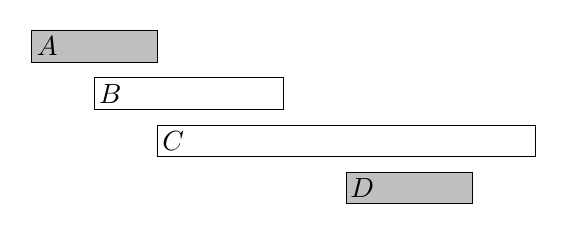
\begin{tikzpicture}[scale=.4]
  \begin{scope}
    \draw[fill=lightgray] (2, 0) rectangle (6, -1);
    \draw (4, -1.5) rectangle (10, -2.5);
    \draw (6, -3) rectangle (18, -4);
    \draw[fill=lightgray] (12, -4.5) rectangle (16, -5.5);
    \node at (2.5,-0.5) {$A$};
    \node at (4.5,-2) {$B$};
    \node at (6.5,-3.5) {$C$};
    \node at (12.5,-5) {$D$};
  \end{scope}
\end{tikzpicture}
\end{center}

このアルゴリズムは常に最適解を生成することができます。
最初にできるだけ早く終了するイベントを選択することが常に最適な選択です。
その後、同じ戦略で次のイベントを選択しそれ以上のイベントを選択できなくなるまで続けることが最適な選択となります。

このアルゴリズムを証明する一つの方法を示します。
最初にできるだけ早く終わる事象より、遅く終わる事象を選択した場合にどうなるかを考えてみましょう。
次のイベントの選択の仕方は(最大でも)同じ数のイベントの選択肢しかありません。
このため、遅く終わるイベントを選択してもより良い解が得られることはないので貪欲なアルゴリズムが正しいということになります。

\section{締め切り付きタスク問題 - Tasks and deadlines}

期間と期限を持つ$n$個のタスクが与えられ、
タスクの実行順序を選択する問題を考えてみます。
ここで各タスクについて$d - x$点のスコアを獲得するとします。
$d$はタスクの期限$x$であるタスクが終了した時点とします。

例えば、以下のようなタスクがあるとする。
\begin{center}
\begin{tabular}{lll}
タスク & 期間 & 期限 \\
\hline
$A$ & 4 & 2 \\
$B$ & 3 & 5 \\
$C$ & 2 & 7 \\
$D$ & 4 & 5 \\
\end{tabular}
\end{center}

最適解は以下の通りです。

\begin{center}
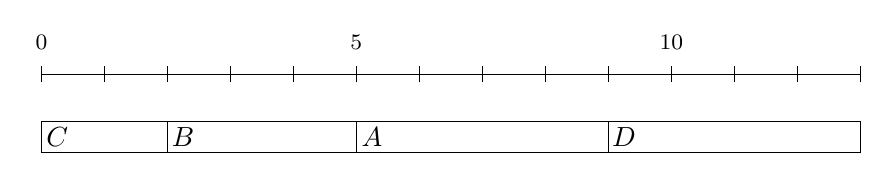
\begin{tikzpicture}[scale=.4]
  \begin{scope}
    \draw (0, 0) rectangle (4, -1);
    \draw (4, 0) rectangle (10, -1);
    \draw (10, 0) rectangle (18, -1);
    \draw (18, 0) rectangle (26, -1);
    \node at (0.5,-0.5) {$C$};
    \node at (4.5,-0.5) {$B$};
    \node at (10.5,-0.5) {$A$};
    \node at (18.5,-0.5) {$D$};

    \draw (0,1.5) -- (26,1.5);
    \foreach \i in {0,2,...,26}
    {
        \draw (\i,1.25) -- (\i,1.75);
    }
    \footnotesize
    \node at (0,2.5) {0};
    \node at (10,2.5) {5};
    \node at (20,2.5) {10};

  \end{scope}
\end{tikzpicture}
\end{center}

この解答では、Cが$5$点、Bが$0$点、Aが$-7$点、Dが$-8$点で合計で-10点となります。

意外なことに、この問題の最適解は期限に全く依存せず、
単にタスクにかかる時間順に並べたタスクを実行することが正しい貪欲な戦略となります。
その理由は、2つのタスクを次々に実行して最初のタスクが2番目のタスクより時間がかかるようなことがあれば、
タスクを入れ替えた方が良くなるからです。
例えば、次のようなスケジュールを考えてみます。

\begin{center}
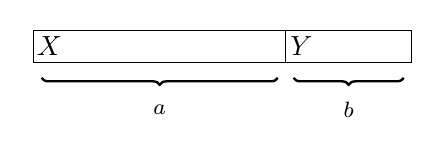
\begin{tikzpicture}[scale=.4]
  \begin{scope}
    \draw (0, 0) rectangle (8, -1);
    \draw (8, 0) rectangle (12, -1);
    \node at (0.5,-0.5) {$X$};
    \node at (8.5,-0.5) {$Y$};

\draw [decoration={brace}, decorate, line width=0.3mm] (7.75,-1.5) -- (0.25,-1.5);
\draw [decoration={brace}, decorate, line width=0.3mm] (11.75,-1.5) -- (8.25,-1.5);

\footnotesize
\node at (4,-2.5) {$a$};
\node at (10,-2.5) {$b$};

  \end{scope}
\end{tikzpicture}
\end{center}
ここでは、$a>b$なので、タスクを入れ替える必要があります
\begin{center}
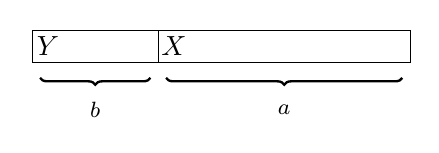
\begin{tikzpicture}[scale=.4]
  \begin{scope}
    \draw (0, 0) rectangle (4, -1);
    \draw (4, 0) rectangle (12, -1);
    \node at (0.5,-0.5) {$Y$};
    \node at (4.5,-0.5) {$X$};

\draw [decoration={brace}, decorate, line width=0.3mm] (3.75,-1.5) -- (0.25,-1.5);
\draw [decoration={brace}, decorate, line width=0.3mm] (11.75,-1.5) -- (4.25,-1.5);

\footnotesize
\node at (2,-2.5) {$b$};
\node at (8,-2.5) {$a$};

  \end{scope}
\end{tikzpicture}
\end{center}

今、$X$は$b$を獲得し、$Y$は$a$を獲得します。
このため、$a-b > 0$となります。
最適解では、連続する2つのタスクについて、
短いタスクが長いタスクの前に来ることが成立しなければいけません。
従って、タスクはその時間順に並べられなければなりません。

\section{最小和問題 - Minimizing sums}

ここで、 $n$ 個の整数$a_1,a_2,\ldots,a_n$
が与えられたときに、次の和が最小になる$x$を求めたいとします。
\[|a_1-x|^c+|a_2-x|^c+\cdots+|a_n-x|^c.\]
ここでは、$c=1$ と $c=2$を例にとります。

\subsubsection{Case $c=1$}

この場合は次の通りです。
\[|a_1-x|+|a_2-x|+\cdots+|a_n-x|.\]
$[1,2,9,2,6]$を入力とすると、最適な解は$x=2$
の時で、
\[
|1-2|+|2-2|+|9-2|+|2-2|+|6-2|=12.
\]
となります。

一般的な場合、$x$は数字の\textit{median - 中央値}、つまりソート後の真ん中の数字が最適となります。。
例えば,$[1,2,9,2,6]$ というリストは,並べ替えの結果 $[1,2,2,6,9]$ なので,中央値である 2 を選びます。

$x$が中央値より小さければ、
$x$を大きくすれば合計は小さくなり、
$x$が中央値より大きければ、
$x$を小さくすれば合計は小さくなるから、
最適解は$x$が中央値となります。
$n$が偶数で中央値が2つある場合は両方の値および、その間のすべての値が最適な選択となります。

\subsubsection{Case $c=2$}

この場合は次の最小化です。
\[(a_1-x)^2+(a_2-x)^2+\cdots+(a_n-x)^2.\]
例えば、数字が$[1,2,9,2,6]$の場合、最適な解は $x = 4$ を選択することで、この場合、
和は次のようになります。
\[
(1-4)^2+(2-4)^2+(9-4)^2+(2-4)^2+(6-4)^2=46.
\]
一般的な場合に、$x$は数字の平均を選ぶのが最適です。
この例では、$(1+2+9+2+6)/5=4$です。
この結果は、次のように和を提示することで導き出すことができる。
\[
nx^2 - 2x(a_1+a_2+\cdots+a_n) + (a_1^2+a_2^2+\cdots+a_n^2)
\]
最後の部分は$x$に依存しないので、ここでは無視してもよいです。
残りの部分は$s=a_1+a_2+\cdots+a_n$に対して、関数 $nx^2-2xs$ を形成します。
これは $x = 0$ と $x = 2s/n$ の根を持つ上に開く放物線(訳註:二次関数)になるため、
最小値は$x=s/n$で、これは$a_1,a_2,\ldots,a_n$の平均となります。

\section{データ圧縮 - Data compression}

\index{データ圧縮 - data compression}
\index{バイナリコード - binary code}
\index{codeword}

\key{バイナリコード - binary code}とは、
文字列の各文字に、ビットで構成される\key{コードワード - codeword}を割り当てたものです。
各文字を対応するコードワードに置き換えることで、バイナリコードを使って文字列を圧縮することができます。
例えば、次のバイナリコードでは、文字\texttt{A}–\texttt{D}にコードワードを割り当てています。

\begin{center}
\begin{tabular}{rr}
character & codeword \\
\hline
\texttt{A} & 00 \\
\texttt{B} & 01 \\
\texttt{C} & 10 \\
\texttt{D} & 11 \\
\end{tabular}
\end{center}
これは各コードワードの長さが同じであることを意味する\key{定長 - constant-length}符号と呼ばれます。
例えば、\texttt{AABACDACA}という文字列を圧縮する場合、次のようになります。
\[00\,00\,01\,00\,10\,11\,00\,10\,00\]
この符号を用いると、圧縮される文字列の長さは18ビットです。
コードワードの長さが異なる\key{可変長 - variable-length}符号を用いると、
文字列をより圧縮することができます。
よく登場する文字には短いコードワードを与え、めったに登場しない文字には長いコードワードを与えていきます。
上記の文字列に対する最適な符号は、次のようになります。

\begin{center}
\begin{tabular}{rr}
character & codeword \\
\hline
\texttt{A} & 0 \\
\texttt{B} & 110 \\
\texttt{C} & 10 \\
\texttt{D} & 111 \\
\end{tabular}
\end{center}
最適な符号は、可能な限り短い圧縮文字列を生成でき、最適な符号を用いた圧縮文字列は
\[0\,0\,110\,0\,10\,111\,0\,10\,0,\]
と、18ビットではなく15ビットになり3ビットを節約することができました。

コードワードは他のコードワードの接頭辞でないように決めることが重要です。
例えば、あるコードが10と1011の両方のコードワードを含むことは許されません。
この理由は、圧縮された文字列から元の文字列を生成できるようにしたいからです。
もしコードワードが他のコードワードの接頭辞になり得るとしたら、これは常に可能とは限りません。

たとえば、次のようなコードワードにしてはいけません。
\begin{center}
\begin{tabular}{rr}
character & codeword \\
\hline
\texttt{A} & 10 \\
\texttt{B} & 11 \\
\texttt{C} & 1011 \\
\texttt{D} & 111 \\
\end{tabular}
\end{center}
圧縮された文字列1011が文字列\texttt{AB}に対応するのか、文字列\texttt{C}に対応するのかが区別できないからです。

\index{ハフマン符号化 - Huffman coding}

\subsubsection{ハフマン符号化 - Huffman coding}

\key{ハフマン符号化 - Huffman coding}
\footnote{D. A. Huffman discovered this method
when solving a university course assignment
and published the algorithm in 1952 \cite{huf52}.}
は、与えられた文字列を圧縮するために最適な符号を構築す る貪欲なアルゴリズムです。
このアルゴリズムは、文字列中の文字の頻度をもとに二分木を構築し、
根から対応するノードへのパスを辿り各文字のコードワードを読み取ります。
左への移動はビット0に対応し、右への移動はビット1に対応します。

初期状態では、文字列の各文字は、
その文字が文字列中に出現する回数を重みとするノードで表現します。
次に、各ステップで重みが最小の2つのノードが結合され、
元のノードの重みの合計を重みとする新しいノードを作成します。
この処理をすべてのノードが結合されるまで続けます。

実際に\texttt{AABACDACA}という文字列に対して、
ハフマン符号化がどのように最適な符号を生成するかを見ていきましょう。
最初に、文字列の文字に対応する4つのノードが存在します。
\begin{center}
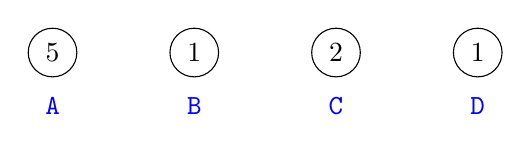
\begin{tikzpicture}[scale=0.9]
\node[draw, circle] (1) at (0,0) {$5$};
\node[draw, circle] (2) at (2,0) {$1$};
\node[draw, circle] (3) at (4,0) {$2$};
\node[draw, circle] (4) at (6,0) {$1$};

\node[color=blue] at (0,-0.75) {\texttt{A}};
\node[color=blue] at (2,-0.75) {\texttt{B}};
\node[color=blue] at (4,-0.75) {\texttt{C}};
\node[color=blue] at (6,-0.75) {\texttt{D}};

%\path[draw,thick,-] (4) -- (5);
\end{tikzpicture}
\end{center}

文字\texttt{A}は文字列中に5回出現するので、文字\texttt{A}を表すノードの重みは5です。
他の重みも同じように計算されます。

まず、重さ1の文字\texttt{B}と文字\texttt{D}に対応するノードを結合した結果がこれです。
\begin{center}
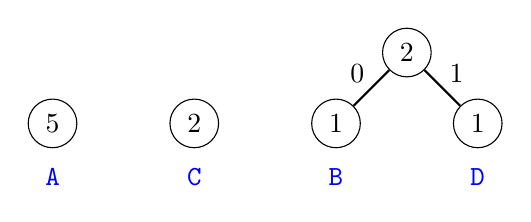
\begin{tikzpicture}[scale=0.9]
\node[draw, circle] (1) at (0,0) {$5$};
\node[draw, circle] (3) at (2,0) {$2$};
\node[draw, circle] (2) at (4,0) {$1$};
\node[draw, circle] (4) at (6,0) {$1$};
\node[draw, circle] (5) at (5,1) {$2$};

\node[color=blue] at (0,-0.75) {\texttt{A}};
\node[color=blue] at (2,-0.75) {\texttt{C}};
\node[color=blue] at (4,-0.75) {\texttt{B}};
\node[color=blue] at (6,-0.75) {\texttt{D}};

\node at (4.3,0.7) {0};
\node at (5.7,0.7) {1};

\path[draw,thick,-] (2) -- (5);
\path[draw,thick,-] (4) -- (5);
\end{tikzpicture}
\end{center}
重み2のノードを結合します。
\begin{center}
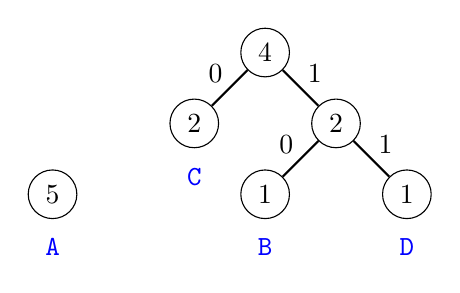
\begin{tikzpicture}[scale=0.9]
\node[draw, circle] (1) at (1,0) {$5$};
\node[draw, circle] (3) at (3,1) {$2$};
\node[draw, circle] (2) at (4,0) {$1$};
\node[draw, circle] (4) at (6,0) {$1$};
\node[draw, circle] (5) at (5,1) {$2$};
\node[draw, circle] (6) at (4,2) {$4$};

\node[color=blue] at (1,-0.75) {\texttt{A}};
\node[color=blue] at (3,1-0.75) {\texttt{C}};
\node[color=blue] at (4,-0.75) {\texttt{B}};
\node[color=blue] at (6,-0.75) {\texttt{D}};

\node at (4.3,0.7) {0};
\node at (5.7,0.7) {1};
\node at (3.3,1.7) {0};
\node at (4.7,1.7) {1};

\path[draw,thick,-] (2) -- (5);
\path[draw,thick,-] (4) -- (5);
\path[draw,thick,-] (3) -- (6);
\path[draw,thick,-] (5) -- (6);
\end{tikzpicture}
\end{center}
最後に残った2つのノードを結合します。
\begin{center}
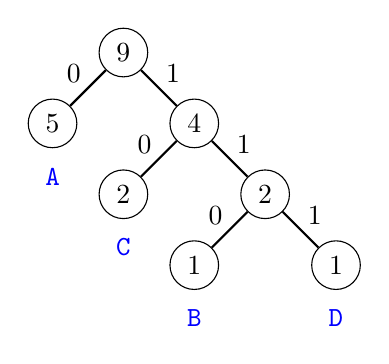
\begin{tikzpicture}[scale=0.9]
\node[draw, circle] (1) at (2,2) {$5$};
\node[draw, circle] (3) at (3,1) {$2$};
\node[draw, circle] (2) at (4,0) {$1$};
\node[draw, circle] (4) at (6,0) {$1$};
\node[draw, circle] (5) at (5,1) {$2$};
\node[draw, circle] (6) at (4,2) {$4$};
\node[draw, circle] (7) at (3,3) {$9$};

\node[color=blue] at (2,2-0.75) {\texttt{A}};
\node[color=blue] at (3,1-0.75) {\texttt{C}};
\node[color=blue] at (4,-0.75) {\texttt{B}};
\node[color=blue] at (6,-0.75) {\texttt{D}};

\node at (4.3,0.7) {0};
\node at (5.7,0.7) {1};
\node at (3.3,1.7) {0};
\node at (4.7,1.7) {1};
\node at (2.3,2.7) {0};
\node at (3.7,2.7) {1};

\path[draw,thick,-] (2) -- (5);
\path[draw,thick,-] (4) -- (5);
\path[draw,thick,-] (3) -- (6);
\path[draw,thick,-] (5) -- (6);
\path[draw,thick,-] (1) -- (7);
\path[draw,thick,-] (6) -- (7);
\end{tikzpicture}
\end{center}

すべてのノードがツリー上に揃ったので、コードワードをツリーから読み取りましょう。
\begin{center}
\begin{tabular}{rr}
character & codeword \\
\hline
\texttt{A} & 0 \\
\texttt{B} & 110 \\
\texttt{C} & 10 \\
\texttt{D} & 111 \\
\end{tabular}
\end{center}
